\documentclass{beamer}
\usepackage{graphicx}


\usetheme{m}
\title{Predicting TCP/IP Network Traffic using Time Series Forecasting}
\date{April 14, 2016}
\author{Thomas Mauerhofer, and Matthias Wölbitsch}


\begin{document}
  \maketitle
  
  \begin{frame}{Motivation}   
    \textbf{TCP/IP networks} 
    \begin{itemize}
      \item telecommunication networks (e.g. WANs)
      \item internet: collection of networks 
      \item cruicial part of todays infrastructure  
      \item various applications depend on it (e.g. banking, \ldots)
    \end{itemize}
    
    \hspace{10pt}
    
    \textbf{\(\rightarrow\) important to understand and forecast behaviour}
  \end{frame}
  
  \begin{frame}{Motivation}
    \textbf{Internet Service Provider (ISP)}
    \begin{itemize}
     \item optimize ressources
     \item improve quality of service
    \end{itemize}
    
    \textbf{Network Security}
    \begin{itemize}
     \item detecting anomalies in network traffic
     \item examples: DDoS attacks, spam floods
     \item compare observed with expected traffic
     \item early detection
    \end{itemize}    
  \end{frame}


  \begin{frame}{Dataset}
    \textbf{Part of the Time Series Data Libary}
    \begin{itemize}
     \item large collection of time series datasets
     \item by Rob Hyndman
    \end{itemize}

    \textbf{Data from private european ISP}
    \begin{itemize}
     \item traffic passing through transantlantic link
    \end{itemize}

    \textbf{Key Characteristics}
    \begin{itemize}
     \item three different resolutions (5 minutes, hourly, and daily)
     \item collected between June 7th and July 31th 2005
    \end{itemize}

  \end{frame}

  \begin{frame}{Dataset}
   \textbf{Time Series Plots (???)}
   \begin{figure}
       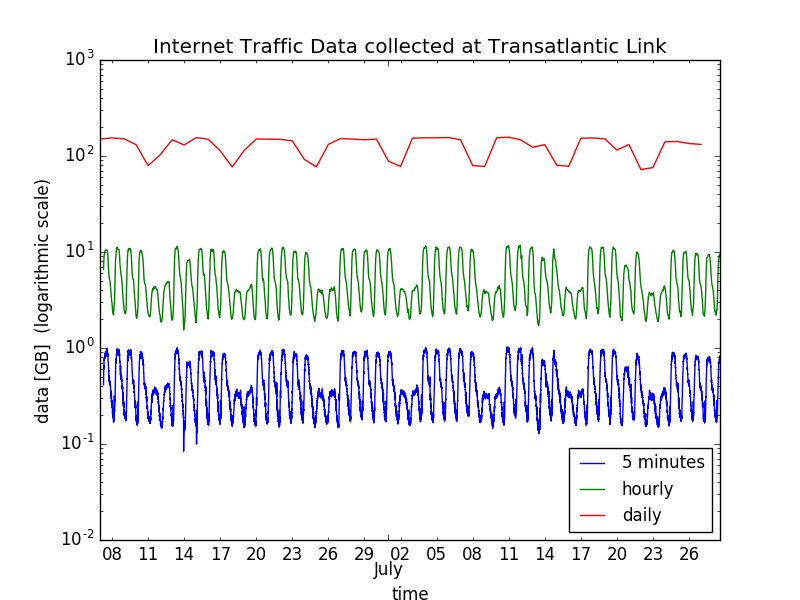
\includegraphics[width=0.8\textwidth]{images/datasets.png}
       \caption{Time series plots with three different resolutions.}
      \end{figure}
  \end{frame}
  
  \begin{frame}{Dataset}   
    \textbf{Weekly and Daily Patterns}
    \begin{columns}[c]
      \column{0.5\textwidth}  
      \begin{figure}
       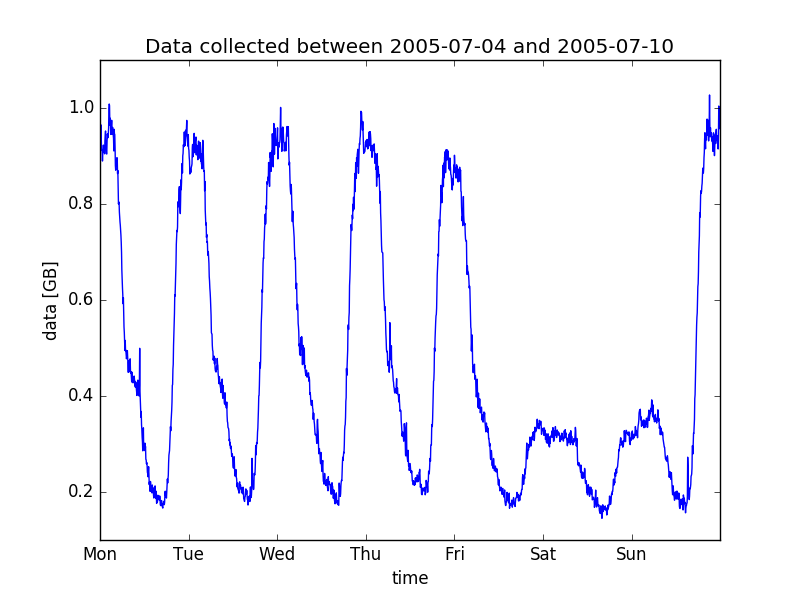
\includegraphics[width=1.05\textwidth]{images/traffic_over_week.png}
       \caption{Typical pattern of a single week.}
      \end{figure}

      \column{0.5\textwidth}
        \begin{figure}
         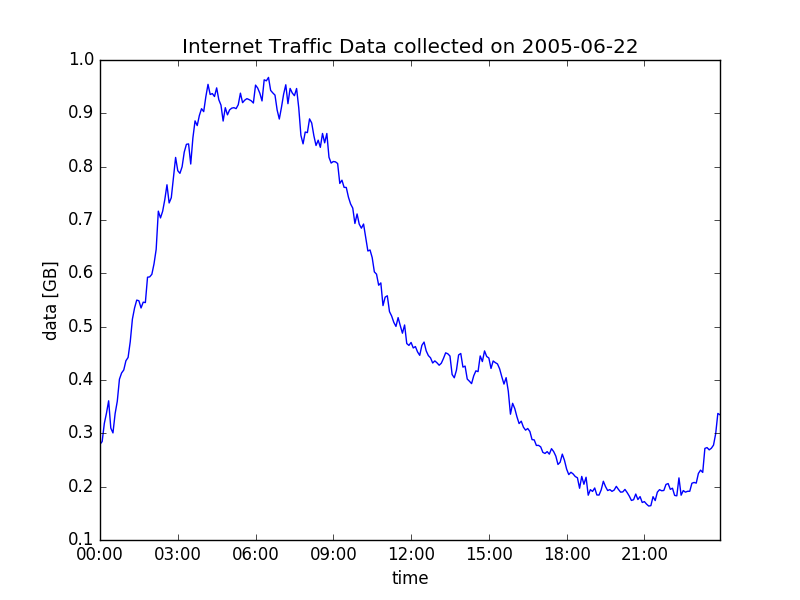
\includegraphics[width=1.05\textwidth]{images/traffic_over_day.png}
         \caption{Typical pattern of a single day.}
        \end{figure}
    \end{columns}
  \end{frame}  
  
    \begin{frame}{Dataset}   
    \textbf{Autocorrelation Plots}
    \begin{columns}[c]
      \column{0.5\textwidth}  
      \begin{figure}
       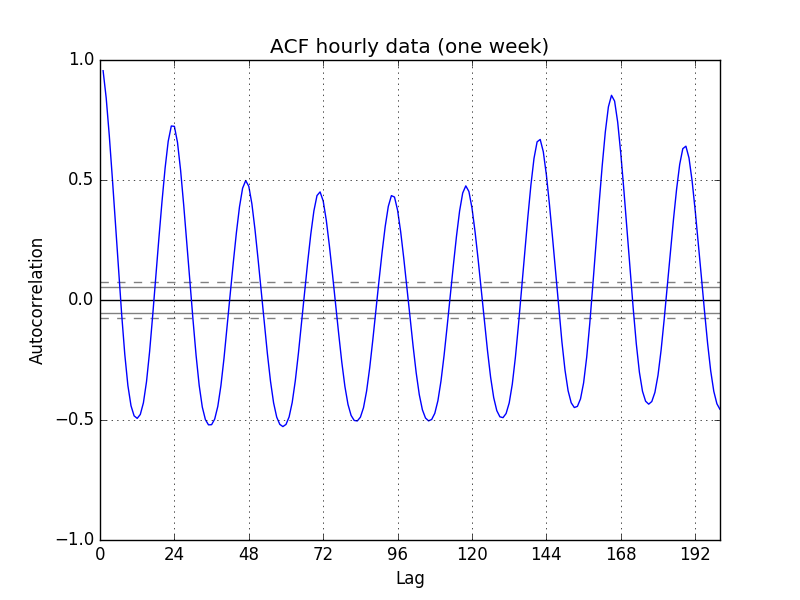
\includegraphics[width=1.05\textwidth]{images/ACF_week.png}
       \caption{ACF which shows daily and weekly patterns based on hourly data.}
      \end{figure}

      \column{0.5\textwidth}
        \begin{figure}
         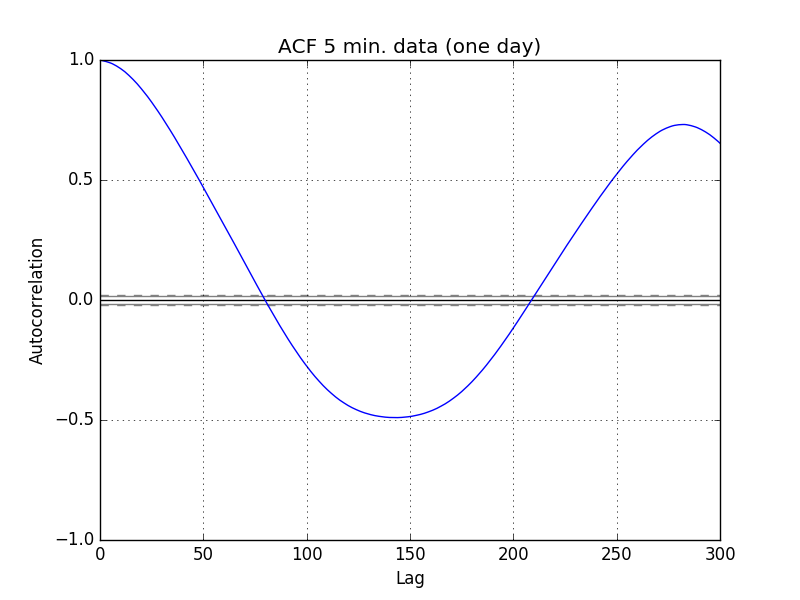
\includegraphics[width=1.05\textwidth]{images/ACF_day.png}
         \caption{ACF which shows daily pattern using the 5 minute data.}
        \end{figure}
    \end{columns}
  \end{frame}  
  
  \plain{Questions?}
  
\end{document}